\documentclass[11 pt ]{article}
\usepackage[utf8]{inputenc}
\usepackage{caption}
\usepackage{subcaption}
\usepackage{url}

\usepackage{ifpdf}
\ifpdf
\usepackage[pdftex]{graphicx}
\else
\usepackage{graphicx}
\fi

\usepackage[margin=1.15 in]{geometry}


\title{6.830 Final Project Report \\ Hive Join Optimization}
\author{Kainar Kamalov, Maksim Stepanenko, Tiffany Lin}

\date{May 2012}

\begin{document}


\setlength{\baselineskip}{1.3\baselineskip}

\ifpdf
\DeclareGraphicsExtensions{.pdf, .jpg, .tif}
\else
\DeclareGraphicsExtensions{.eps, .jpg}
\fi

\maketitle

\section{Introduction}
Hive is a data warehouse infrastructure built on top of Hadoop for providing data for summarization, query, and analysis. In this project we tried two different approaches to optimizing Hive's join algorithm. The first approach is based on the estimated cost model computed during the runtime, and the second approach is based on the estimation of the hash table growth in order to make decisions. To see the benefit of our optimizations we compared the optimized system's performance with the original version using our constructed join-heavy queries and the data generated for TPC-H benchmark \cite{tpc-h}. In the remainder of this paper first we are going to discuss Hive's current join algorithm implementation and the relevant parts of its architecture. Next we will present and discuss the results of running TPC-H benchmark on Hive's original implementation. After that we will talk about the two methods we used to optimize the algorithm and the results they produced, we will also compare them to the results produced by the original implementation. We will conclude by summarizing our TPC-H benchmark, and the optimization results and by discussing if the optimizations we implemented were worthwhile for the given workloads.
\section{Hive Architecture and Join Algorithm}
In this section we will discuss the way join operations work in Hive and describe the architecture responsible for them. Hive is an infrastructure on top of Hadoop (an open-source implementation of Google's Map-Reduce framework); it compiles SQL queries into map-reduce jobs and runs them in a cluster. Since join is one of the most heavily used SQL operations and since often it is the bottleneck in the performance of query processing, we decided to look into optimizing it. Currently the join operation on Hive consists of two different options for executing a join operation: Common Join Task and Map Join Task. 
\subsection{Common Join Task}
\begin{figure}
	      \centering
                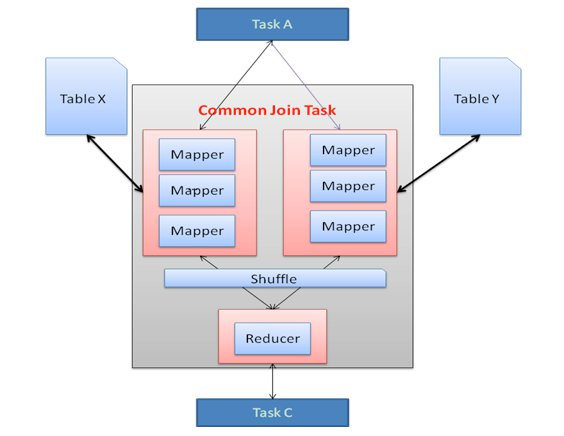
\includegraphics[scale=0.6]{common.jpg}
              \caption{Common Join Task \cite{facebook-join}}
              \label{fig:common-join}
\end{figure}

A common join task compiles into a regular map-reduce job with both map and reduce stages, as shown in Figure~\ref{fig:common-join}. In the mapping stage the mappers read the tables and emit <key, value> pairs, indexed on the join attribute, into intermediate files. The shuffler then reads all the emitted pairs and sorts them by the key. The reducers read the sorted data and do the actual join work. The bottleneck of this approach is the shuffling stage, since all the data needs to be sorted and merged, before the reducers can start the join operation.

\subsection{Map Join Task}
A Map Join Task is motivated by the fact that the shuffling stage in the Common Join Task takes a lot of time, and sometimes it is completely unnecessary, especially in the case when the tables are small. As shown in Figure~\ref{fig:map-join}, the Map Join Task is completed by the mappers and thus doesn't need the shuffle and reduce stages. When at least one of the tables is small enough to fit into memory, mappers can just read it in and do the work locally, in memory. The small table is processed by the Map-Reduce Local Task and the resulting hash table, index by the key, is the pushed in to the Distributed Cache. All the mappers then have access to the hash table and can execute the Map Join by reading the small table data from the Distributed Cache and the large table data from HDFS. All the joining happens inside the mappers in this approach, thus eliminating the expensive shuffle stage, when unnecessary. 
\begin{figure}
	      \centering
                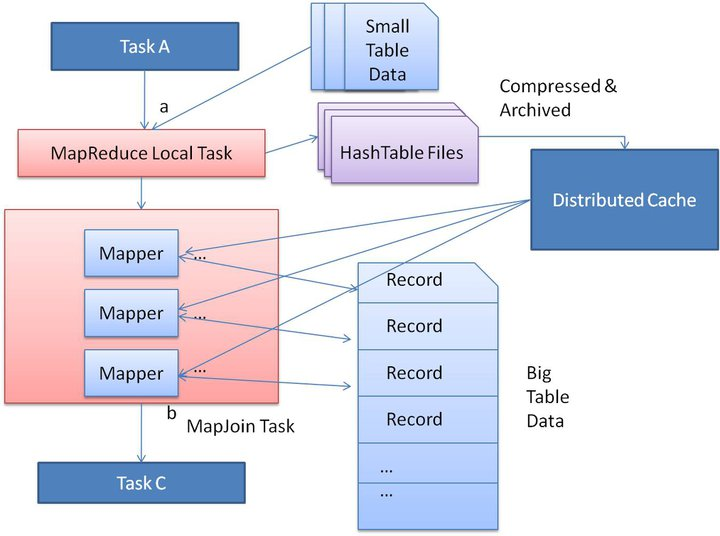
\includegraphics[scale=1]{mapjoin.jpg}
              \caption{Map Join Task \cite{facebook-join}}
              \label{fig:map-join}
\end{figure}

\subsection{Conditional Task}
Given the two different join strategies, described above, the system has to be able to decide when to use one over the other. Clearly Map Join cannot be used with large tables, because the hash table will not fit in memory, so there will be even more overhead from storing part of it to HDFS and then retrieving it back; on the other hand, the Common Join is not very efficient when at least one of the tables is small enough to fit in memory and introduces a lot of unnecessary overhead. The purpose of the Conditional Task is to decide, given the available at runtime table information, whether to use Common Join or Map Join. Figure~\ref{fig:conditional} shows the high-level view of how all the components are used together in Hive. The current Hive implementation uses a very simple condition to make the decision in the Conditional Task: if one of the tables is $\leq 25$ MB, then the Map Join is used, otherwise the Common Join task is fired up. 25 MB is a very conservative factor and will not always result in the most optimal decision. For example, the table, although of small size, might have a very large number of tuples, in which case the hash tables will grow too large to fit in memory and thus the performance will actually be worse than with Common Join. In the next paragraphs we will describe two different decision frameworks for the Conditional Task that we implemented and will also talk about their effect on the performance of the join operation.
\begin{figure}
	      \centering
                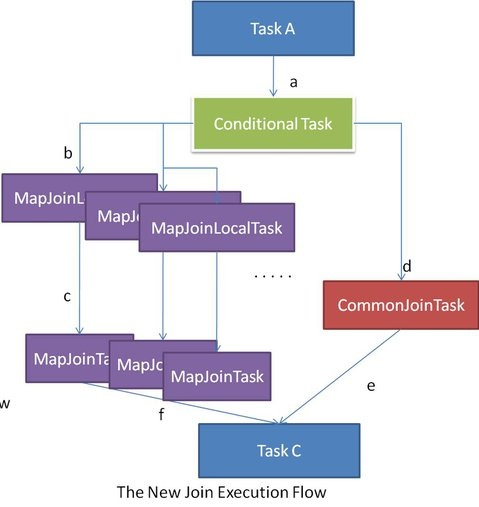
\includegraphics[scale=1]{condition.jpg}
              \caption{ Task \cite{facebook-join}}
              \label{fig:conditional}
\end{figure}
\section{Cost Model Estimation}
In this section we will describe the first optimization of the decision framework that takes into account the state of the entire join architecture when deciding which join task to use. Instead of just using the hardcoded 25 MB estimate, we decided to make an estimation of this number in a more programmatic way by calculating it from the cost model that we developed for the join processing architecture. We developed two cost models for both of the join tasks available and attempted to make the estimation using them. While developing these models we had to make a number of assumptions, listed below:

\begin{itemize}
\item Assumption 1 KAINAR
\item Assumption 2
\item Assumption 3
\end{itemize}
\subsection{Common Join Cost Model}
The common join cost model gives an approximate time that Common Join will take if it is run for the given join operation. 
EXPLAIN THE REST HERE KAINAR

\subsection{Map Join Cost Model}
The map join cost model approximates the time that would be required if Map Join were to be used for the current join task.  When using Map Join the size of the hash table produced by the Local Map Join task is one of the most important values for the cost model. Because of the way hash tables are implemented in Java, it is hard to precisely calculate the size of the hash table given the small table, so we decided to run a number of experiments and empirically identify the relationship between the contents of the small table and the size of the resulting hash table.
EXPLAIN THE REST HERE KAINAR
\subsection{Performance}
We ran a number of join-heavy queries and obtained the results presented in Table~\ref{tab:cost-table}. As we can see from the results of our performance tests bla bla bla KAINAR
\begin{table}
\centering
\begin{tabular}{ | l | c | r |}
  \hline                        
  Something & Something & Something \\
  \hline
  1 & 2 & 3 \\
    \hline	
  4 & 5 & 6 \\
    \hline
  7 & 8 & 9 \\
  \hline  
\end{tabular}
\caption{Cost Model Performance Evaluation}
\label{tab:cost-table}
\end{table}
\section{Hive Hash Table Growth Estimation}
In this section we are going to describe the second approach that we tried in order to optimize the way the Conditional Task makes decisions. Since the limitation of the Map Join is the fact that it can only handle the tables that will produce a hash table small enough to fit in memory, we decided to try a different approach. Rather than using the cost model, which takes into account all the components of the process, we decided to just focus on the growth of the hash table based on the contents of the small table. Because of large overheads that Java introduces with the objects, it is hard to calculate the size of the hash table precisely. We used the relationship we found earlier in the first approach to estimate the size of the hash table given the contents of the small table. In this approach we make a decision by calculating a threshold on the number of rows the small table can have, by estimating the size of the hash table these rows will produce.

\subsection{Growth Estimation}
talk here about how we do the estimation of the tables KAINAR
\subsection{Performance}
To see the effect of our modifications we ran a number of join-heavy queries on the data that was generated by TPC-H framework. The results are presented in Table~\ref{tab:hashtable-table}. As we can see from the results bla bla bla KAINAR
\begin{table}
\centering
\begin{tabular}{ | l | c | c | r |}
  \hline                        
  Something & Something & Something & something \\
  \hline
  1 & 2 & 3 & 4\\
    \hline	
  4 & 5 & 6 & 5\\
    \hline
  7 & 8 & 9 & 6\\
  \hline  
\end{tabular}
\caption{Cost Model Performance Evaluation}
\label{tab:hashtable-table}
\end{table}
\section{TPC-H Benchmark Results}
In this section we will show the results of running TPC-H benchmark on the original implementation of Hive. 
bla bla bla KAINAR
\section{Discussion and Conclusion}
KAINAR if you want to, otherwise I can write this after you are done with the other sections, so I have some results to write about :P

\bibliographystyle{plain}
\begin{thebibliography}{77}
\bibitem{tpc-h}
\url{http://www.tpc.org/tpch/}

\bibitem{facebook-join}
\author{Liyin Tang},
\url{https://www.facebook.com/note.php?note_id=470667928919}

\end{thebibliography}

\bibliography{}

\end{document}

